\lecture{7}{2025-10-27}{}

\section{Chomsky Normal Form}

We want to simplify the structure of context-free grammars. One useful normal form is the Chomsky Normal Form (CNF).

\begin{definition}[Chomsky Normal Form]
    A context-free grammar is in \textbf{Chomsky Normal Form} if all its production rules are of the form:
    \begin{itemize}
        \item \(A \to BC\), where \(A, B, C\) are non-terminal symbols and \(B, C\) are not the start symbol.
        \item \(A \to a\), where \( a \in \Sigma \) (\( \varepsilon \notin \Sigma \))
        \item \(S \to \varepsilon\) is allowed, where \(S\) is the start symbol.
    \end{itemize}
\end{definition}    

\begin{eg}
    Convert the following CFG to CNF:
    \begin{align*}
        S &\to ASA \mid aB \\
        A &\to B \mid S \\
        B &\to b \mid \varepsilon
    \end{align*}
\end{eg}

First, we add $S_0$ as the new start symbol:
\[
    S_0 \to S \quad  S \to ASA \mid aB \quad A \to B \mid S \quad B \to b \mid \varepsilon
\]
Next, we remove the $\varepsilon$-productions $B \to \varepsilon$:
\[
    S_0 \to S \quad S \to ASA \mid aB \mid \red{a} \quad A \to B \mid \red{\varepsilon} \mid S \quad B \to b
\]
Next, we remove the $\varepsilon$-productions $A \to \varepsilon$:
\[
    S_0 \to S \quad S \to ASA \mid aB \mid a \mid \red{AS} \mid \red{SA} \mid \red{S} \quad A \to B \mid S \quad B \to b
\]
Next, we remove single production $S \to S$:
\[
    S_0 \to S \quad S \to ASA \mid aB \mid a \mid AS \mid SA \quad A \to B \mid S \quad B \to b
\]
Next, we remove single production $S_0 \to S$:
\[
    S_0 \to \red{ASA \mid aB \mid a \mid AS \mid SA} \quad S \to ASA \mid aB \mid a \mid AS \mid SA \quad A \to B \mid S \quad B \to b
\]
Next, we remove single production $A \to B$, $A \to S$:
\[
    S_0 \to ASA \mid aB \mid a \mid AS \mid SA \quad S \to ASA \mid aB \mid a \mid AS \mid SA \quad A \to \red{b \mid ASA \mid aB \mid a \mid AS \mid SA} \quad B \to b
\]
Finally, we convert to CNF by introducing new variables for terminals and breaking down long productions:
\begin{align*}
    S_0 &\to AA_1 \mid U B \mid a \mid A S \mid S A \\
    S &\to AA_1 \mid U B \mid a \mid A S \mid S A \\
    A &\to b \mid AA_1 \mid U B \mid a \mid A S \mid S A \\
    A_1 &\to SA \\
    B &\to b \\
    U &\to a
\end{align*}

\subsection{Procedure of Converting CFG to CNF}
To convert any CFG to CNF, we can follow these steps:
\begin{enumerate}[label=$\arabic*^\circ$]
    \item \textbf{Add} a new start symbol \(S_0\) with the production \[S_0 \to S\]
    \item \textbf{Remove} all \(\varepsilon\)-productions, except for the start symbol, i.e. \(A \to \varepsilon \ (A \neq S_0)\), for any 
    \[
        \cdots \to uAv
    \]
    add the production
    \[
        \cdots \to u v
    \]
    \item \textbf{Remove} single productions of $A \to B$ where \(A, B \in V/\{S\} \). 
    \[
        A \to B, \ B \to \gamma \quad \implies \quad A \to \gamma
    \]
    \begin{remark}
        $A \to \gamma$ can't be a unit rule previously removed.
    \end{remark}
    \item \textbf{Convert} remaining productions to CNF:
    \[
        A \to u_1 u_2 \cdots u_k \quad u_i \in V \cup \Sigma
    \]
    and
    \[
        \text{if } k = 1, \text{ then } u_i \in \Sigma
    \]
    Convert as follows:
    \begin{align*}
        A &\to u_1 A_1 \\
        A_1 &\to u_2 A_2 \\
        &\vdots
    \end{align*}
    Replaced every terminal \(u_i \in \Sigma\) with a new variable \(U_i\):
    \[
        U_i \to u_i \quad u_i \in \Sigma
    \]
\end{enumerate}

\subsection{Infinite Loop in Converting}
\begin{eg}
    Consider the grammar:
    \begin{align*}
        S &\to B \mid \varepsilon \\
        B &\to S \mid \varepsilon
    \end{align*}
\end{eg}

We first add a new start symbol:
\[
    S_0 \to S \quad S \to B \mid \varepsilon \quad B \to S \mid \varepsilon
\]
Next, we remove the \(\varepsilon\)-productions:
\[
    S_0 \to S \mid \varepsilon \quad S \to B \quad B \to S \mid \varepsilon
\]
Next, we remove the \(\varepsilon\)-productions again:
\[
    S_0 \to S \mid \varepsilon \quad S \to B \mid \varepsilon \quad B \to S
\]

This process will continue indefinitely. The reason is $S \to \varepsilon$ has been handled. So there is no need to add $S \to \varepsilon$.

\section{Pushdown Automata}

We now introduce the machine that recognizes context-free languages (CFL), called Pushdown Automata (PDA). PDA is a machine with a \red{stack}, which is a way to store previous states.

\begin{figure}[H]
    \centering
    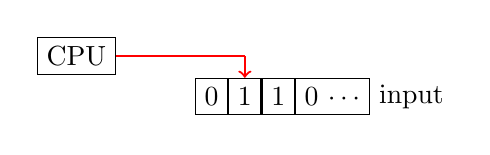
\begin{tikzpicture}[ampersand replacement=\&]
        \matrix 
        {
        \node[draw](0) {CPU}; \& [1cm] \& \node(1){}; \&\&\& \\
        \& \node[draw]{0}; \& \node[draw](a){1}; \& \node[draw]{1}; \& \node[draw]{0 $\cdots$};  \& \node{input};\\
        };
        \draw [-,red,thick] (0) -- (1.center) ;
        \draw [->,red,thick] (1.center) -- (a) ;
    \end{tikzpicture}
    \caption{DFA or NFA}
\end{figure}

\begin{figure}[H]
    \centering
    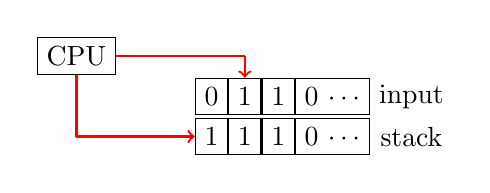
\begin{tikzpicture}[ampersand replacement=\&]
    \matrix 
    {
    \node[draw](0) {CPU}; \& [1cm]  \& \node(1){} ; \&\&\& \\
    \& \node[draw]{0}; \& \node[draw](a){1}; \& \node[draw]{1}; \& \node[draw]{0 $\cdots$};  \& \node{input};\\
    \node(c){}; \& \node[draw](b){1}; \& \node[draw]{1}; \& \node[draw]{1}; \& \node[draw]{0 $\cdots$}; \&  \node{stack}; \\
    };

    \draw [-,red,thick] (0) -- (1.center) ;
    \draw [->,red,thick] (1.center) -- (a) ;
    \draw [-,red,thick] (0) -- (c.center) ;
    \draw [->,red,thick] (c.center) -- (b) ;
    \end{tikzpicture}
    \caption{Pushdown Automata (PDA)}
\end{figure}

\begin{eg}
    Consider the language \(A = \{0^n 1^n \mid n \geq 0\}\). We can design a PDA to recognize \(A\):
\end{eg}

\begin{figure}[H]
    \centering
    \begin{tikzpicture}[node distance=2.5cm, ->, >=Stealth, on grid, auto]
    \node[state,initial,accepting] (q_1) {$q_1$};
    \node[state] (q_2) [right of=q_1] {$q_2$};
    \node[state] (q_3) [below of=q_2] {$q_{3}$};
    \node[state,accepting] (q_4) [left of=q_3] {$q_{4}$};      
    \path 
    (q_1) edge[above]  node {$\varepsilon, \varepsilon \rightarrow \$ $} (q_2)
    (q_2) edge[loop right]  node {$0,\varepsilon \rightarrow 0$} (q_2)
    (q_2) edge[right]  node {$1, 0 \rightarrow \varepsilon$} (q_3)
    (q_3) edge[loop right]  node {$1, 0 \rightarrow \varepsilon$} (q_3)  
    (q_3) edge[below] node {$\varepsilon, \$ \rightarrow \varepsilon$} (q_4);
    \end{tikzpicture}
    \caption{PDA for \(A = \{0^n 1^n \mid n \geq 0\}\)}
\end{figure}

$\$$ is a special bottom stack symbol to indicate the initial state of the stack. The PDA works as follows:

\begin{itemize}
    \item $q_2 \rightarrow q_2$, put 0 into stack
    \item $q_2 \rightarrow q_3$ and $q_3 \rightarrow q_3$, read 1 and \texttt{pop} 0 up
\end{itemize}

If the input is $0011$ which is same as $\varepsilon 0011 \varepsilon$, the process is as follows:
\begin{equation*}
    \begin{split}
    & q_1, \emptyset, \varepsilon\\
    & q_2, \{\$\}, 0 \\
    & q_2, \{0,\$\}, 0\\
    & q_2, \{0,0,\$\}, 1\\
    & q_3, \{0,\$\}, 1\\
    & q_3, \{\$\}, \varepsilon\\
    & q_4, \{\}
    \end{split}
\end{equation*}
\begin{notation}
    $\{\}$: contents of the stack before processing the input character.
\end{notation}

\newpage

\subsection{Formal definition of PDA}

\begin{definition}[Pushdown Automata]
    A \textbf{pushdown automaton} (PDA) is a 6-tuple \((Q, \Sigma, \Gamma, \delta, q_0, F)\), where
    \begin{itemize}
        \item \(Q\): States
        \item \(\Sigma\): Input alphabet
        \item \(\Gamma\): Stack alphabet
        \item \(\delta\): Transition function
        \[
            Q \times \Sigma_{\varepsilon} \times \Gamma_{\varepsilon} \to \mathcal{P}(Q \times \Gamma_{\varepsilon})
        \]
        \item \(q_0 \in Q\): Start state
        \item \(F \subset Q\): Set of accepting states
    \end{itemize}
\end{definition}

The definition of the above PDA for \(A = \{0^n 1^n \mid n \geq 0\}\) is as follows:
\begin{itemize}
    \item \(Q = \{q_1, q_2, q_3, q_4\}\)
    \item \(\Sigma = \{0, 1\}\)
    \item \(\Gamma = \{0, \$\}\)
    \item \(q_0 = q_1\)
    \item \(F = \{q_1, q_4\}\)
\end{itemize}
For the the transition function, we care about three things:
\begin{itemize}
    \item Current state
    \item Current input
    \item \red{Top of the stack}
\end{itemize}
The transition function \(\delta\) works as follows:
\begin{center}
    \begin{tabular}{@{}l|ccc|ccc|ccc@{}}
    & \multicolumn{3}{c|}{0} 
    & \multicolumn{3}{c|}{1} 
        & \multicolumn{3}{c}{$\varepsilon$} \\ \hline
        & 0 & \$ & $\varepsilon$ 
        & 0 & \$ & $\varepsilon$ 
        & 0 & \$ & $\varepsilon$ \\ \hline
        $q_1$ &  &  &  
              &  &  &  
              &  &  & $\{(q_2,\$)\}$ \\
        $q_2$ &  &  & $\{(q_2,0)\}$ 
              & $\{(q_3,\varepsilon)\}$ &  &  
              &  &  &  \\
        $q_3$ &  &  &  
              & $\{(q_3,\varepsilon)\}$ &  &  
              & $\{(q_4,\varepsilon)\}$ &  &  \\
        $q_4$ &  &  &  
              &  &  &  
              &  &  &  \\
    \end{tabular}
\end{center}

For example, we say the transition of $q_2 \to q_3$ to be \[
    \delta(q_2, 1, 0) = \{(q_3, \varepsilon)\}
\]

\subsection{Nondeterministic situation}

\begin{eg}
    Design a PDA for the language \(B = \{a^i b^j c^k \mid i, j, k \geq 0 \text{ and } i = j \text{ or } j = k\}\).
\end{eg}

\begin{figure}[H]
    \centering
    \begin{tikzpicture}[node distance=2.5cm, ->, >=Stealth, on grid, auto]
    \node[state,initial] (q_1) {$q_1$};
    \node[state] (q_2) [right of=q_1] {$q_2$};
    \node[state] (q_3) [above right of=q_2] {$q_{3}$};
    \node[state,accepting] (q_4) [right of=q_3] {$q_{4}$};
    \node[state] (q_5) [below right of=q_2] {$q_{5}$};
    \node[state] (q_6) [right of=q_5] {$q_{6}$};      
    \node[state,accepting] (q_7) [right of=q_6] {$q_{7}$};      
    
    \path 
    (q_1) edge[above]  node {$\varepsilon, \varepsilon \rightarrow \$ $} (q_2)
    (q_2) edge[loop above]  node {$a,\varepsilon \rightarrow a$} (q_2)
    (q_2) edge[right]  node {$\varepsilon, \varepsilon \rightarrow \varepsilon$} (q_3)
    (q_2) edge[right]  node {$\varepsilon, \varepsilon \rightarrow \varepsilon$} (q_5)
    (q_3) edge[loop above]  node {$b, a \rightarrow \varepsilon$} (q_3)
    (q_3) edge[above]  node {$\varepsilon, \$ \rightarrow \varepsilon$} (q_4)
    (q_4) edge[loop above]  node {$c, \varepsilon \rightarrow \varepsilon$} (q_4)
    (q_5) edge[loop below]  node {$b, \varepsilon \rightarrow \varepsilon$} (q_5)
    (q_5) edge[below]  node {$\varepsilon, \varepsilon \rightarrow \varepsilon$} (q_6)
    (q_6) edge[loop below]  node {$c, a \rightarrow \varepsilon$} (q_6)
    (q_6) edge[below] node {$\varepsilon, \$ \rightarrow \varepsilon$} (q_7);
    \end{tikzpicture}
    \caption{Nondeterministic PDA}
\end{figure}

We input $a^2bc^2$, to illustrate the process, we can build the following computation tree:

\begin{center}
    
    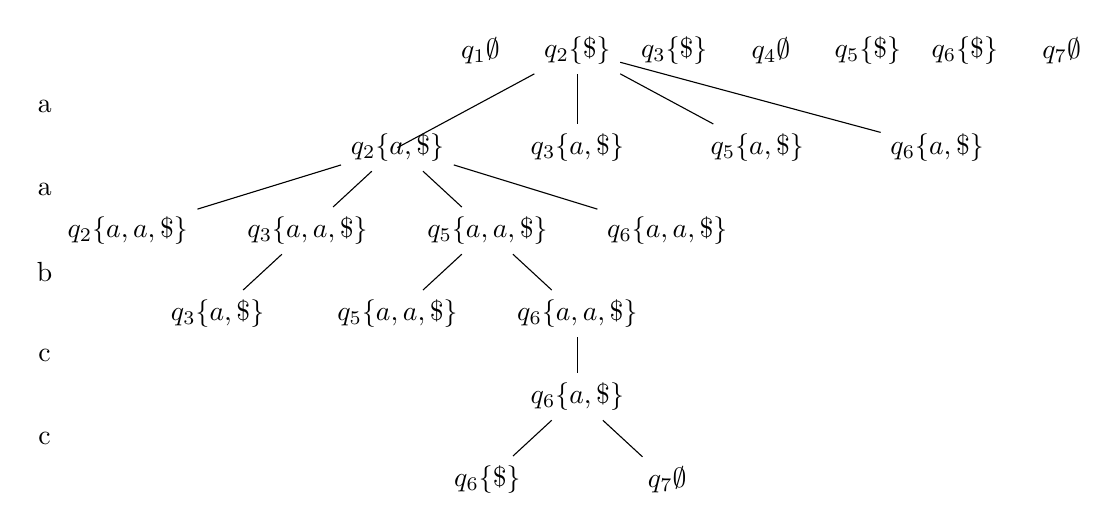
\begin{tikzpicture} [level distance=25pt,sibling distance=65pt]% grow=right
    \node  {$q_1\emptyset$}
    child [grow=right, level distance=35pt] { node  { $q_2\{\$\}$ } edge from parent[draw=none]
      [grow=down]
      child [grow=right] { [level distance=35pt] node  {$q_3\{\$\}$} edge from parent[draw=none]
        child [grow=right] {node  {$q_4\emptyset$} edge from parent[draw=none]
          child [grow=right] {node  {$q_5\{\$\}$} edge from parent[draw=none]
            child [grow=right] {node  {$q_6\{\$\}$} edge from parent[draw=none]
              child [grow=right] {node  {$q_7\emptyset$} edge from parent[draw=none]
              }
            }
          }
        }
      }
      child { [level distance=30pt] node  {$q_2\{a,\$\}$}
        child {node  {$q_2\{a,a,\$\}$}
          child [grow=left] {node (3) {} edge from parent[draw=none]
            child [grow=up] {node (2) {} edge from parent[draw=none]
              child [grow=up] {node (1) {} edge from parent[draw=none]
              }
            }
            child [grow=down] {node (4) {} edge from parent[draw=none]
              child [grow=down] {node (5) {} edge from parent[draw=none]
                child [grow=down] {node (6) {} edge from parent[draw=none]
                }
              }
            }
          }
        }
        child {node  {$q_3\{a,a,\$\}$}
          child {node  {$q_3\{a,\$\}$}
          }
          child {edge from parent[draw=none]}      
        }
        child {node  {$q_5\{a,a,\$\}$}
          child {node  {$q_5\{a,a,\$\}$}}
          child {node  {$q_6\{a,a,\$\}$}
            child {node  {$q_6\{a,\$\}$}
              child {node  {$q_6\{\$\}$}}
              child {node  {$q_7\emptyset$}}
            }
          }
        }
        child {node  {$q_6\{a,a,\$\}$}}
      }    
      child  {node {$q_3\{a,\$\}$}}      
      child  {node {$q_5\{a,\$\}$}}
      child  {node {$q_6\{a,\$\}$}}
    };
    \path (1) -- (2) node [midway] {a};
    \path (2) -- (3) node [midway] {a};
    \path (3) -- (4) node [midway] {b};
    \path (4) -- (5) node [midway] {c};
    \path (5) -- (6) node [midway] {c};
    \end{tikzpicture}
\end{center}

\begin{eg}
    Design a PDA for the language \(C = \{ww^R \mid w \in \{0, 1\}^*\}\).
\end{eg}

\begin{idea}
    Symbols pushed to stack, nondeterministically guess middle is reached
\end{idea}
\begin{figure}[H]
    \centering
    \begin{tikzpicture}[node distance=2.5cm, ->, >=Stealth, on grid, auto]
    \node[state,initial,accepting] (q_1) {$q_1$};
    \node[state] (q_2) [right of=q_1] {$q_2$};
    \node[state] (q_3) [below of=q_2] {$q_{3}$};
    \node[state,accepting] (q_4) [left of=q_3] {$q_{4}$};      
      \path 
      (q_1) edge[above]  node {$\varepsilon, \varepsilon \rightarrow \$ $} (q_2)
      (q_2) edge[loop right]  node {
        \begin{tabular}{l}
          $0,\varepsilon \rightarrow 0$\\
          $1,\varepsilon \rightarrow 1$
        \end{tabular}
    } (q_2)
      (q_2) edge[right]  node {\red{$\varepsilon, \varepsilon \rightarrow \varepsilon$}} (q_3)
      (q_3) edge[loop right]  node {
        \begin{tabular}{l}
          $0, 0 \rightarrow \varepsilon$
          \\
          $1, 1 \rightarrow \varepsilon$
        \end{tabular}
    } (q_3)  
      (q_3) edge[below] node {$\varepsilon, \$ \rightarrow \varepsilon$} (q_4);
    \end{tikzpicture}
    \caption{PDA for \(C = \{ww^R \mid w \in \{0, 1\}^*\}\)}
\end{figure}

\newpage

\subsection{Converting CFL to PDA}
\begin{eg}
    Convert the CFG \(G\) to PDA that recognizes \(L(G)\):
    \begin{align*}
        S &\to aTb \mid b \\
        T &\to Ta \mid \varepsilon
    \end{align*}
\end{eg}

\begin{idea}
    For rule substitution, we replace the left-hand side variable with the right-hand side string
    i.e. 
    \[
        A \to \gamma \quad \implies \quad \text{\texttt{pop} } A \text{ from stack, \texttt{push} } \gamma \text{ to stack}
    \]
    if there are multiple productions for \(A\), we \texttt{push} them \red{in a reversed way}.
\end{idea}

\begin{figure}[H]
    \centering
    \begin{tikzpicture}[node distance=2.5cm, ->, >=Stealth, on grid, auto]
    \node[state,initial] (q_1) {$q_s$};
    \node[state] (q_2) [below of=q_1,yshift=0.5cm] {};
    \node[state] (q_3) [below of=q_2,yshift=0.5cm] {$q_{\text{loop}}$};
    \node[state] (q_4) [above right of=q_3, yshift=0.5cm, xshift=0.5cm] {$q_1$};
    \node[state] (q_6) [right of=q_4, yshift=2.0cm] {$q_2$};
    \node[state] (q_5) [below right of=q_3, yshift=0.6cm, xshift=2.5cm] {$q_3$};
    \node[state] (q_7) [below of=q_3,yshift=0.5cm,accepting] {$q_a$};
      \path 
      (q_1) edge[left]  node {$\varepsilon, \varepsilon \rightarrow \$ $} (q_2)
      (q_2) edge[left]  node {$\varepsilon, \varepsilon \rightarrow S $} (q_3)
      (q_3) edge[left]  node {$\varepsilon, \$ \rightarrow \varepsilon $} (q_7)    
      (q_3) edge[loop left]  node [xshift=-0.2cm] {
        \begin{tabular}{l}
          $\varepsilon,S \rightarrow b$\\
          $\varepsilon, T \rightarrow \varepsilon$\\
          \red{$a, a \rightarrow \varepsilon$}\\
          \red{$b, b \rightarrow \varepsilon$}
        \end{tabular}
      } (q_3)
      (q_3) edge[right]  node {$\varepsilon, S \rightarrow b$} (q_4)
      (q_4) edge[right]  node {$\varepsilon, \varepsilon \rightarrow T$} (q_6)
      (q_6) edge[bend right, above]  node {$\varepsilon, \varepsilon \rightarrow a$} (q_3)
      (q_3) edge[below, bend left]  node {$\varepsilon, T \rightarrow a$} (q_5)
      (q_5) edge[below, bend left]  node {$\varepsilon, \varepsilon \rightarrow T$} (q_3)  
    ;
    \end{tikzpicture}
    \caption{PDA for CFG \(G\)}
\end{figure}

\begin{remark}
    There are two transitions we must add to process the "input":
    \begin{align*}
        a, a &\to \varepsilon \\
        b, b &\to \varepsilon
    \end{align*}
\end{remark}

The procedure of converting CFG to PDA is as follows:
\begin{eqnarray*}
&& q_{\text{start}} \stackrel{\varepsilon}{\rightarrow}
q_{\text{loop}}, \{S,\$\} 
\stackrel{\varepsilon}{\rightarrow} q_1, \{b,\$\}
\stackrel{\varepsilon}{\rightarrow} q_2, \{T,b,\$\} \\
&& \stackrel{\varepsilon}{\rightarrow} q_{\text{loop}}, \{a,T,b,\$\} 
\stackrel{\red{a}}{\rightarrow}
 q_{\text{loop}}, \{T,b,\$\} \\
&& \stackrel{\varepsilon}{\rightarrow} q_{3}, \{a, b,\$\} 
\stackrel{\varepsilon}{\rightarrow} q_{\text{loop}}, \{T,a,b,\$\}\\
&& \stackrel{\varepsilon}{\rightarrow} q_3, \{a,a,b,\$\}
\stackrel{\varepsilon}{\rightarrow} q_{\text{loop}}, \{T,a,a,b,\$\}\\
&& \stackrel{\varepsilon}{\rightarrow} q_3, \{a,a,a,b,\$\}
\stackrel{\varepsilon}{\rightarrow} q_{\text{loop}}, \{T,a,a,a,b,\$\}\\
&& \stackrel{\varepsilon}{\rightarrow} q_{\text{loop}}, \{a,a,a,b,\$\}
\stackrel{a}{\rightarrow} q_{\text{loop}}, \{a,a,b,\$\}\\
&& \stackrel{a}{\rightarrow} q_{\text{loop}},\{a,b,\$\}
\stackrel{a}{\rightarrow} q_{\text{loop}}, \{b,\$\}\\
&& \stackrel{b}{\rightarrow} q_{\text{loop}}, \{\$\}
\stackrel{\varepsilon}{\rightarrow} q_{accept}
\end{eqnarray*}

\newpage

\begin{proposition}
    Even with a non-deterministic setting, we ensure that only strings generated by this CFG can be accepted by the PDA
    \begin{itemize}
        \item A string is accepted only if all characters are processed (this is part of the PDA definition!)
        \item We have \$ to ensure that the stack is empty in the end
    \end{itemize}
\end{proposition}

\subsection{Converting PDA to CFL}

\begin{lemma}
    Language recognized by PDA $\Longrightarrow$ context free
\end{lemma}

\begin{note}
    We need PDA to satisfy
    \begin{enumerate}[label=$\arabic*^\circ$]
        \item Single start state
        \item Stack empty before accepting
        \item Each transition \texttt{push} or \texttt{pop}, but not both
    \end{enumerate}
\end{note}

\begin{idea}
    For each pair of states \(p, q \in Q\) of a PDA $P$, we have $A_{pq}$ and
    \[
        A_{pq} \text{ generates } x \implies P \text{ from } p \text{ with empty stack to } q \text{ with empty stack, reading } x 
    \]
\end{idea}

First, we discuss how to handle transitions
\[
    \forall p, q, r \in Q, \ A_{pq} \to A_{pr}A_{rq}
\]

We let the
\begin{itemize}
    \item $x$-axis: input string
    \item $y$-axis: stack height
\end{itemize}

\begin{figure}[H]
    \centering
    \begin{tikzpicture}[node distance=2.5cm, ->, >=Stealth, on grid, auto]
        \draw[] (-0.2,0) -- (6,0);
        \draw[] (0,-0.2) -- (0,3.5);
        \draw[-] (0,0) .. controls (2,3.5) .. (3.5, 0);
        \draw[-] (3.5, 0) .. controls (3.8, 2) .. (5.5,0);
        \draw[draw=none] (0,-0.3) node {$p$};
        \draw[draw=none] (3.5,-0.3) node {$r$};
        \draw[draw=none] (5.5,-0.3) node {$q$};
    \end{tikzpicture}
    \caption{PDA transition $A_{pq} \to A_{pr}A_{rq}$}
\end{figure}

If we can go
\begin{center}
    from $p$ to $r$ without changing stack
\end{center}
and
\begin{center}
    from $r$ to $q$ without changing stack
\end{center}
then we can do
\begin{center}
    from $p$ to $q$ without changing stack
\end{center}

\newpage

Next, we have
\[
    \forall p, q, r, s \in Q, \ a, b \in \Sigma_{\varepsilon}, \ t \in \Gamma
\]
If, 
\[
    (r, t) \in \delta(p, a, \varepsilon) \text{ and } (q, \varepsilon) \in \delta(s, b, t)
\]
we discuss how to handle transitions
\[
    A_{pq} \to a A_{rs} b
\]

Then we have 
\begin{figure}[H]
    \centering
    \begin{tikzpicture}[node distance=2.5cm, ->, >=Stealth, on grid, auto]
        \draw[] (-0.2,0) -- (6,0);
        \draw[] (0,-0.2) -- (0,3.5);
        \draw[-] plot [smooth] coordinates { (0,0) (0.55,1) (2,3.4) (3.1, 1.3) (4.2, 2.8) (5.05, 1 ) (5.5,0)};
        \draw[-,dashed] (0.55,1) -- (0.55,0);
        \draw[-,dashed] (5.05,1) -- (5.05,0);
        \draw[draw=none] (-0.2,-0.3) node {$p$};
        \draw[draw=none] (0.3,-0.3) node {$a$};
        \draw[draw=none] (5.3,-0.3) node {$b$};
        \draw[draw=none] (5.7,-0.3) node {$q$};
        \draw[draw=none] (0.8,1) node {$r$};
        \draw[draw=none] (0.8,0.45) node {$t$};
        \draw[draw=none] (4.8,1) node {$s$};
        \draw[draw=none] (4.8,0.45) node {$t$};
    \end{tikzpicture}
    \caption{PDA transition $A_{pq} \to a A_{rs} b$}    
\end{figure}

Finally, we have the following base case:
\[
    \forall p \in Q, \ A_{pp} \to \varepsilon
\]

To follow the condition ($1^\circ$), we give a new example
\begin{eg}
    Consider the language \(L = \{0^n 1^n \mid n \geq 1\}\).
\end{eg}
Now $q_1$ is not an accept state

\begin{figure}[H]
    \centering
    \begin{tikzpicture}[node distance=2.5cm, ->, >=Stealth, on grid, auto]
    \node[state,initial] (q_1) {$q_1$};
    \node[state] (q_2) [right of=q_1] {$q_2$};
    \node[state] (q_3) [below of=q_2] {$q_{3}$};
    \node[state,accepting] (q_4) [left of=q_3] {$q_{4}$};      
    \path 
    (q_1) edge[above]  node {$\varepsilon, \varepsilon \rightarrow \$ $} (q_2)
    (q_2) edge[loop right]  node {$0,\varepsilon \rightarrow 0$} (q_2)
    (q_2) edge[right]  node {$1, 0 \rightarrow \varepsilon$} (q_3)
    (q_3) edge[loop right]  node {$1, 0 \rightarrow \varepsilon$} (q_3)  
    (q_3) edge[below] node {$\varepsilon, \$ \rightarrow \varepsilon$} (q_4);
    \end{tikzpicture}
    \caption{PDA for \(A = \{0^n 1^n \mid n \geq 1\}\)}
\end{figure}

Consider two elements in \(\Gamma\)
\[
    t_0 = \$, \quad t_1 = 0
\]
\begin{itemize}
    \item $t=\$$
    \begin{center}
    \begin{tabular}{lllllll}
        p & r & s & q & t & a & b\\ \hline
        1 & 2 & 3 & 4 & \$ & $\varepsilon$ & $\varepsilon$
    \end{tabular}
    \end{center}
    then we can get the rule
    \[
        A_{14} \to A_{23}
    \]
    \newpage
    \item $t=0$
    \begin{center}
    \begin{tabular}{lllllll}
        p & r & s & q & t & a & b\\ \hline
        2 & 2 & 2 & 3 & 0 & 0 & 1\\
        2 & 2 & 3 & 3 & 0 & 0 & 1\\
    \end{tabular}
    \end{center}
    then we can get the rules
    \begin{align*}
        A_{23} &\to 0 A_{22} 1 \\
        A_{23} &\to 0 A_{23} 1
    \end{align*}
\end{itemize}

Other rules: 64 rules
\begin{eqnarray*}
&&A_{11}\rightarrow A_{11}A_{11}\\
&&A_{11}\rightarrow A_{12}A_{21}\\
&&A_{11}\rightarrow A_{13}A_{31}\\
&&A_{11}\rightarrow A_{14}A_{41}\\
&&\vdots
\end{eqnarray*}
and
\begin{eqnarray*}
&& A_{11}\rightarrow \varepsilon \\  
&& A_{22}\rightarrow \varepsilon \\
&& A_{33}\rightarrow \varepsilon \\
&& A_{44}\rightarrow \varepsilon 
\end{eqnarray*}

\subsection{Procedure of converting PDA to CFL}
\begin{proposition}
    Given a PDA
    \[
        P=(Q,\Sigma, \Gamma, \delta, q_0, \{q_{accept}\})
    \]
    We construct a CFG with variables
    \[
        \text{var}(G) =\{A_{pq}\mid p, q \in Q\}
    \]
    and start variable
    \[
        S = A_{q_0 q_{accept}}
    \]
    With rules
    \begin{enumerate}[label=$\arabic*^\circ$]
        \item Single start state
        \item Stack empty before accepting
        \item Each transition \texttt{push} or \texttt{pop}, but not both
    \end{enumerate}
    
    A new start $q_s \rightarrow q_{s'}$ with $\varepsilon, \varepsilon \rightarrow \$ $, and for any $q \in F$, we have $\varepsilon, a\rightarrow \varepsilon $ back to $q$, $\forall a \in \Sigma$. Then from any $q \in F$, we do $\varepsilon, \$ \rightarrow \varepsilon$ to $q_a$
\end{proposition}

\newpage

\begin{figure}[H]
    \centering
    \begin{tikzpicture}[node distance=2.5cm, ->, >=Stealth, on grid, auto]
        \node[state,initial] (q_0) {$q_{s'}$};
        \node[state,draw=none,fill=white] (q_d) [right of=q_0, xshift=-1cm] {$\cdots$};    
        \node[state] (q_1) [above right of=q_d, accepting, yshift=-1cm] {$q_1$};
        \node[state] (q_2) [below right of=q_d, accepting, yshift=1cm] {$q_2$};
    \end{tikzpicture}
    \caption{PDA with single accept state and empty stack before accepting}
\end{figure}
The new one will become
\begin{figure}[H]
    \centering
    \begin{tikzpicture}[node distance=2.5cm, ->, >=Stealth, on grid, auto]
        \node[state] (q_0) {$q_{s'}$};
        \node[state,initial above, left of=q_0] (q_s) {$q_{s}$};    
        \node[state,draw=none,fill=white] (q_d) [right of=q_0, xshift=-1.3cm] {$\cdots$};    
        \node[state] (q_1) [above right of=q_d, yshift=-1.2cm,xshift=-0.3cm] {$q_1$};
        \node[state] (q_2) [below right of=q_d, yshift=1.2cm,xshift=-0.3cm] {$q_2$};
        \node[state,accepting, right of=q_d, xshift=2cm] (q_a) {$q_{a}$};

        \path 
        (q_s) edge[above]  node {$\varepsilon, \varepsilon \rightarrow \$ $} (q_0)
        (q_1) edge[loop above]  node {$\varepsilon, a \rightarrow \varepsilon$\quad $\varepsilon, b \rightarrow \varepsilon$ } (q_1)
        (q_2) edge[loop below]  node {$\varepsilon, a \rightarrow \varepsilon$\quad $\varepsilon, b \rightarrow \varepsilon$} (q_2)  
        (q_1) edge[above]  node {$\varepsilon, \$ \rightarrow \varepsilon$} (q_a)
        (q_2) edge[below]  node {$\varepsilon, \$ \rightarrow \varepsilon$} (q_a);
    \end{tikzpicture}
\end{figure}

These is not enough to ensure condition ($3^\circ$), we can do some modifications:
\begin{itemize}
    \item To have each transition either \texttt{push} or \texttt{pop} (but not both), replace
    \[
        q_1 \xrightarrow{a,\, a \rightarrow b} q_2
    \]
    with the pair
    \[
        q_1 \xrightarrow{a,\, a \rightarrow \varepsilon} q_3,
        \qquad
        q_3 \xrightarrow{\varepsilon,\, \varepsilon \rightarrow b} q_2.
    \]
    \item Likewise, replace
    \[
        q_1 \xrightarrow{a,\, \varepsilon \rightarrow \varepsilon} q_2
    \]
    with
    \[
        q_1 \xrightarrow{a,\, \varepsilon \rightarrow X} q_3,
        \qquad
        q_3 \xrightarrow{\varepsilon,\, X \rightarrow \varepsilon} q_2,
    \]
    where $X$ is a fresh stack marker introduced for this simulation.
\end{itemize}

For another example, consider the PDA
\begin{center}
    \begin{tikzpicture}[node distance=2.5cm, ->, >=Stealth, on grid, auto]
        \node[state,initial] (q_0) {$q_{s'}$};
        \node[state] [right of=q_0] (q_1) {$q_{1}$};
        \node[state,accepting] [right of=q_1] (q_2) {$q_{2}$};
        \node[state,accepting] [above=2cm of q_2] (q_3) {$q_{3}$};
        \path[->]
        (q_0) edge [below] node {$\varepsilon,\varepsilon\to a$} (q_1)
        (q_1) edge [below] node {$\varepsilon,\varepsilon\to b$} (q_2)
        (q_2) edge [right] node {$a,a\to\varepsilon$} (q_3)
        ;
    \end{tikzpicture}
\end{center}

After the modification, we have
\begin{center}
\begin{tikzpicture}[node distance=2.5cm, ->, >=Stealth, on grid, auto]
    \node[state,initial right] (q_s) {$q_{s}$};
    \node[state] [below of=q_s](q_0) {$q_{s'}$};
    \node[state] [right of=q_0] (q_1) {$q_{1}$};
    \node[state] [right of=q_1] (q_2) {$q_{2}$};
    \node[state] [above of=q_2] (q_3) {$q_{3}$};
    \node[state,accepting] [right of=q_3] (q_a) {$q_a$};
    \path[->]
    (q_s) edge [right] node {$\varepsilon,\varepsilon\to\$$} (q_0)
    (q_0) edge [below] node {$\varepsilon,\varepsilon\to a$} (q_1)
    (q_1) edge [below] node {$\varepsilon,\varepsilon\to b$} (q_2)
    (q_2) edge [left] node {$a,a\to\varepsilon$} (q_3)
    (q_3) edge [above] node {$\varepsilon,\$\to\varepsilon$} (q_a)
    (q_2) edge [sloped,above] node {$\varepsilon,\$\to\varepsilon$} (q_a)
    (q_3) edge [loop left,left,text width=1.3cm] node {$\varepsilon,a\to\varepsilon$ $\varepsilon,b\to\varepsilon$} (q_3)
    (q_2) edge [loop right,right,text width=2cm] node {$\varepsilon,a\to\varepsilon$ $\varepsilon,b\to\varepsilon$} (q_2)
    ;
\end{tikzpicture}
\end{center}

\newpage

The new PDA will accept the string $a$ but the original PDA rejects it. Hence, we need to modify something else:
\begin{itemize}
    \item A new start $q_s \rightarrow q_{s'}$ with $\varepsilon, \varepsilon
    \rightarrow \$ $
    \item A \red{new state $q_\text{pop}$} that have $\varepsilon,a\rightarrow \varepsilon $ back to $q_\text{pop}$, $\forall a$. 
    \item For $q\in F$, add a transition $\varepsilon,\varepsilon\to\varepsilon$ from $q$ to $q_\text{pop}$
    \item Add a new accept state $q_a$ and a transition $\varepsilon,\$\to\varepsilon$ from $q_\text{pop}$ to $q_a$
\end{itemize}
    
\begin{figure}[H]
    \centering
    \begin{tikzpicture}[node distance=2.5cm, ->, >=Stealth, auto]
        \node[state] (q_0) {$q_{s'}$};
        \node[state,initial above,left of=q_0] (q_s) {$q_{s}$};    
        \node[state,draw=none,fill=white] (q_d) [right=0cm of q_0] {$\cdots$};    
        \node[state] (q_1) [right=-0.3cm of q_d, yshift=2cm] {$q_1$};
        \node[state] (q_2) [right=-0.3cm of q_d, yshift=-2cm] {$q_2$};
        \node[state, right=2cm of q_d] (q_pop) {$q_\text{pop}$};
        \node[state,accepting, right of=q_pop] (q_a) {$q_{a}$};

    \path 
    (q_s) edge[above]  node {$\varepsilon, \varepsilon \rightarrow \$ $} (q_0)
    (q_pop) edge[loop below,text width=2cm]  node {$\varepsilon, a \rightarrow \varepsilon$\quad $\varepsilon, b \rightarrow \varepsilon$} (q_pop)  
    (q_1) edge[above,sloped]  node {$\varepsilon,\varepsilon \rightarrow \varepsilon$} (q_pop)
    (q_2) edge[above,sloped]  node {$\varepsilon,\varepsilon \rightarrow \varepsilon$} (q_pop)
    (q_pop) edge [above] node {$\varepsilon,\$\to\varepsilon$} (q_a)
    ;
    \end{tikzpicture}
    \caption{PDA with single accept state and empty stack before accepting}
\end{figure}

% \section{Deterministic Pushdown Automata}

% \chapter{The Church-Turing Thesis}

% \section{Turing Machines}
% \section{Multitape Turing Machines}
% \section{Nondeterministic Turing Machines}
% \section{Hilbert's problems}

% \chapter{Decidability}

% \section{Decidability}
% \section{Halting Problem}

% \chapter{Reducibility}

% \section{Reducibility}
% \section{Computation Histories}

% \chapter{Complexity Theory}

% \section{Big-O Notation}
% \section{Time Complexity}
% \section{Languages in P}
% \section{Languages in NP}
